\section{Experiments} \label{sec:experiments}
In all our experiments, we train conditional RNNs by unfolding them
up to a certain maximum length. 
We chose this length to cover about $95\%$ of the target sentences in the data sets we consider.
The remaining sentences are cropped to the chosen maximum length. 
For training, we use stochastic gradient descent
with mini-batches of size $32$ and we reset the hidden states at the
beginning of each sequence. Before updating the parameters we
re-scale the gradients if their norm is above $10$~\citep{mikolov-2010}.
We search over the values of hyper-parameter, such as the initial learning rate, 
the various scheduling parameters, number of epochs, \etc, using a held-out validation set. 
We then take the model that performed best on the validation set and compute BLEU or ROUGE 
score on the test set. In the following sections we report results on the test set only. 
Greedy generation is performed by taking the most likely word at each time step.~\footnote{Code available at: \url{https://github.com/facebookresearch/MIXER}} 

\subsection{Text Summarization}
We consider the problem of abstractive summarization where, 
given a piece of ``source" text, we aim at generating its summary (the ``target" text)
such that its meaning is intact.  
The data set we use to train and evaluate our models consists of a 
subset of the Gigaword corpus~\citep{gigaword} as described in~\citet{rush-2015}. 
This is a collection of news articles taken from different sources over the past two decades. 
Our version is organized as a set of example pairs, where each pair is composed of the 
first sentence of a news article (the source sentence) and its corresponding headline (the target sentence). 
We pre-process the data in the same way as in~\citep{rush-2015}, which consists of lower-casing 
and replacing the infrequent words with a special token denoted by ``$<$unk$>$". After 
pre-processing there are $12321$ unique words in the source dictionary and $6828$ words in the target dictionary. The number of sample pairs in the training, validation and test set are $179414$, $22568$, 
and $22259$ respectively. The average sequence length of the target headline is about $10$ words. 
We considered sequences up to $15$ words to comply with our initial constraint of covering at least
$95$\% of the data.

Our generative model is a conditional Elman RNN (Equation~\ref{eq:elman-rnn}) with $128$ hidden units, 
where the conditioning vector $\bc_t$  is provided by a convolutional attentive encoder, 
similar to the one described in Section 3.2 of ~\citet{rush-2015} and inspired by 
\cite{bahdanau-iclr2015}. The details of our attentive 
encoder are mentioned in Section~\ref{sup-material:encoder} of the Supplementary Material.
%The words in the source context are embedded and averaged over
%windows of size $5$, yielding vectors $\bs_t$. 
%Then, the actual context vector $\bc_t$ is computed as a weighted
%sum of these $\bs_t$, where the weights are computed via a
%softmax on the dot products between the current hidden state $\bh_t$
%and the vectors $\bs_t$  themselves, a mechanism known as {\em attention}~\citep{bahdanau-iclr2015}. 
We also tried LSTMs as our generative model for this task, however it did not improve performance. We conjecture this is due to the fact that the target sentences in this data set are rather short.

\subsection{Machine Translation}
For the translation task, our generative model is an LSTM with $256$ hidden units and it uses the same attentive encoder architecture as the one used for summarization. 
We use data from the German-English machine translation track of the
IWSLT 2014 evaluation campaign \citep{cettolo2014}.
The corpus consists of sentence-aligned subtitles of TED and TEDx 
talks. We pre-process the training data using the tokenizer of the Moses 
toolkit \citep{koehn2007} and remove sentences longer than $50$ words as well as casing.  
The training data comprises of about $153000$ sentences where the average English 
sentence is $17.5$ words long and the average German sentence is 
$18.5$ words long. In order to retain at least $95\%$ of this data, we unrolled our RNN for $25$ steps.
Our validation set comprises of $6969$ sentence pairs which was taken from the training data. The test set is a concatenation of dev2010, dev2012, tst2010, tst2011 and tst2012 
which results in $6750$ sentence pairs. The English dictionary has $22822$ words while the German has $32009$ words. 
% /gfsai-oregon/ai-group/datasets/text/iwslt14/de-en/prep_large_valid $ wc *
%     6750   125738   718762 test.de-en.de
%     6750   131141   657528 test.de-en.en
%   153326  2687417 15424177 train.tags.de-en.de
%   153326  2836550 14204700 train.tags.de-en.en
%     6969   122327   701505 valid.de-en.de
%     6969   129091   647345 valid.de-en.en
\subsection{Image Captioning}
For the image captioning task, we use the MSCOCO
dataset~\citep{mscoco}. We use the entire training set provided by the authors, which consists of around $80$k images. We then took the original validation set (consisting of around $40$k images) and randomly sampled (without replacement) $5000$ images for validation and another $5000$ for test. 
There are $5$ different captions for each image. 
At training time we sample one of
these captions, while at test time we report the maximum BLEU score across the five captions.
The context is represented by 1024 features extracted by a Convolutional Neural Network (CNN) trained
on the Imagenet dataset~\citep{imagenet_cvpr09}; we do not back-propagate through these features. We use a similar experimental set up as described in ~\citet{sbengio-nips2015}. The RNN is a single layer LSTM with 
$512$ hidden units and the image features are provided to the generative model as the first word in the sequence. We pre-process the captions by lower-casing all words and replacing all the words which appear less than 3 times with a special token ``$<$unk$>$". As a result the total number of unique words in our dataset is $10012$. Keeping in mind the $95\%$ rule, we unroll the RNN for $15$ steps.

\subsection{Results}
In order to validate MIXER, we compute BLEU score on the machine translation and image captioning task, and ROUGE on the summarization task. 
%For instance, for every document in the test set of the summarization task, we predict the headline and then compute ROUGE with respect to the ground truth title. 
The input provided to the system is only the context and the beginning of sentence token. We apply the same protocol to the baseline methods as well. The scores on the test set are reported in Figure~\ref{fig:gain}. \begin{figure}[!t]
\centering
\begin{minipage}[c][][c]{.4\textwidth}
\centering
%\small
\begin{tabular}{l || l | l | l |l}
\multicolumn{1}{c||}{\emph{TASK} }  & 
      \multicolumn{1}{c|}{XENT} &
      \multicolumn{1}{c|}{DAD} & \multicolumn{1}{c|}{E2E} & \multicolumn{1}{c}{MIXER}\\
      \hline
      \hline
      {\em summarization} & 13.01 & 12.18 & 12.78 &  \bf{16.22} \\
      \hline
      {\em translation} & 17.74 & 20.12 & 17.77 & {\bf 20.73} \\
      \hline
      {\em image captioning} & 27.8 & 28.16 & 26.42 & \bf{29.16} \\
    \end{tabular}
\end{minipage}\hfill
\begin{minipage}[c][][c]{.4\textwidth}
\centering
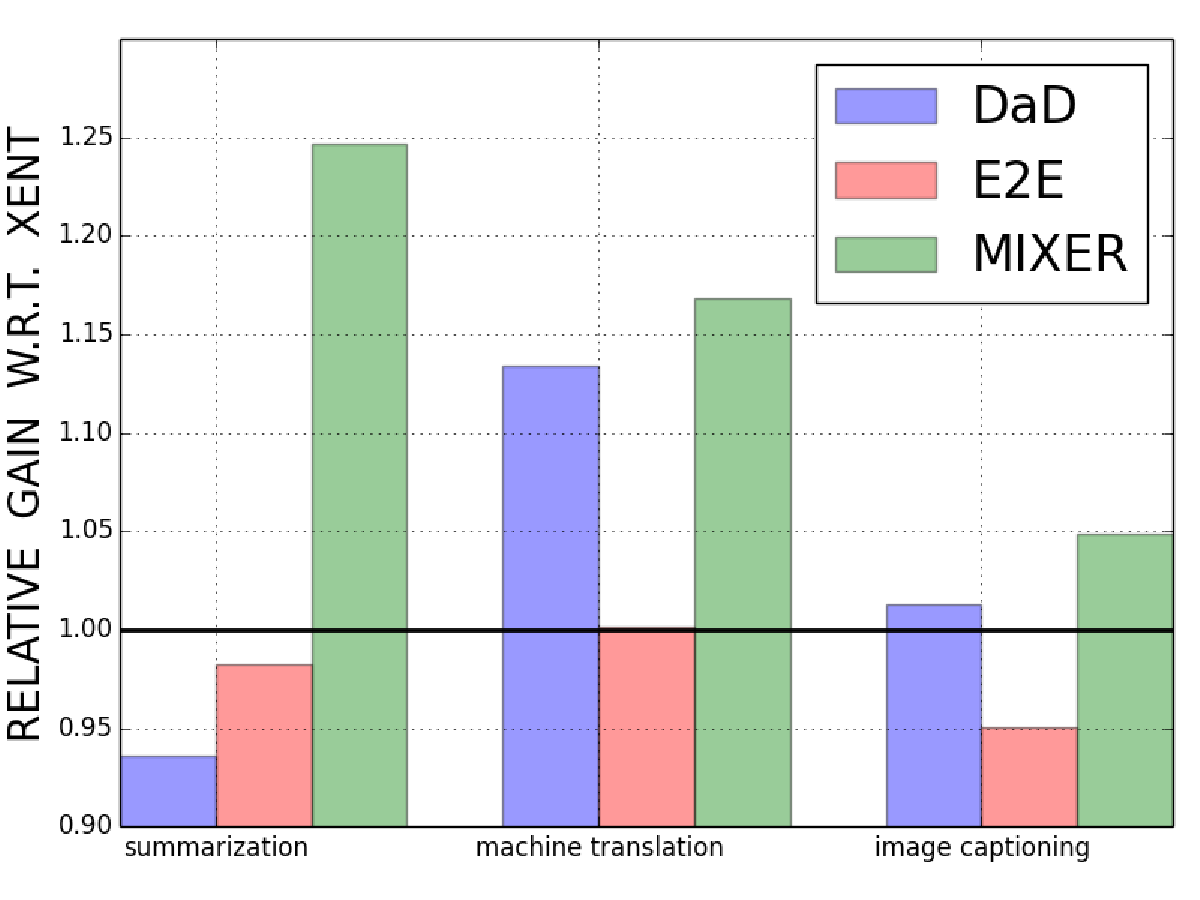
\includegraphics[width=0.8\linewidth]{comparison2.pdf}
\vspace{-.30cm}
\caption{Left: BLEU-4 (translation and image captioning) and ROUGE-2 (summarization) scores using greedy generation. Right: Relative gains
  produced by DAD, E2E and MIXER on the three tasks. 
  The relative gain is computed as the ratio between the score of a model over the score of the reference XENT model on the same task. The horizontal line indicates the performance of XENT.}
\label{fig:gain}
\end{minipage}
\end{figure}
\begin{figure}[!t]
\begin{center}
%\hspace{-.5cm}
 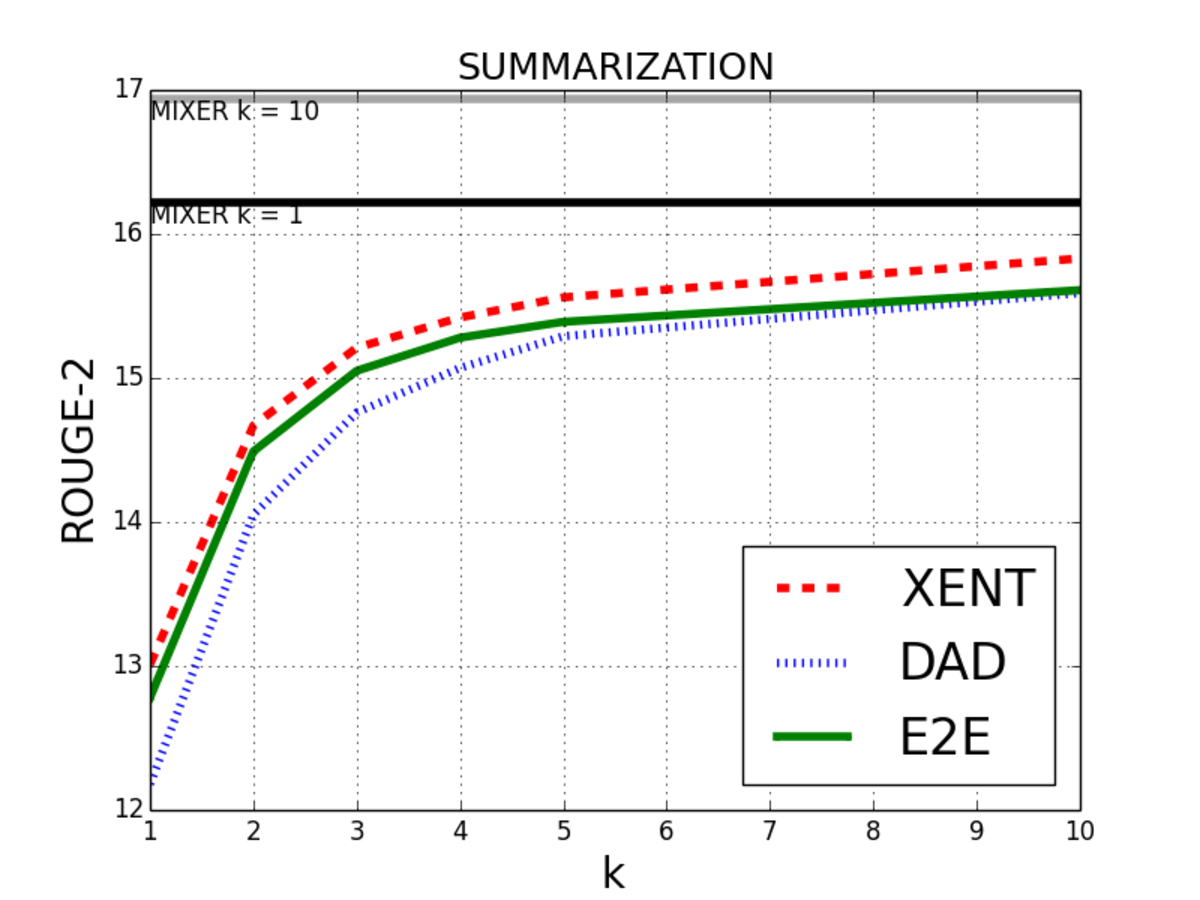
\includegraphics[width=.35\linewidth]{summarization_beamsearch.pdf}
 \hspace{-.6cm}
 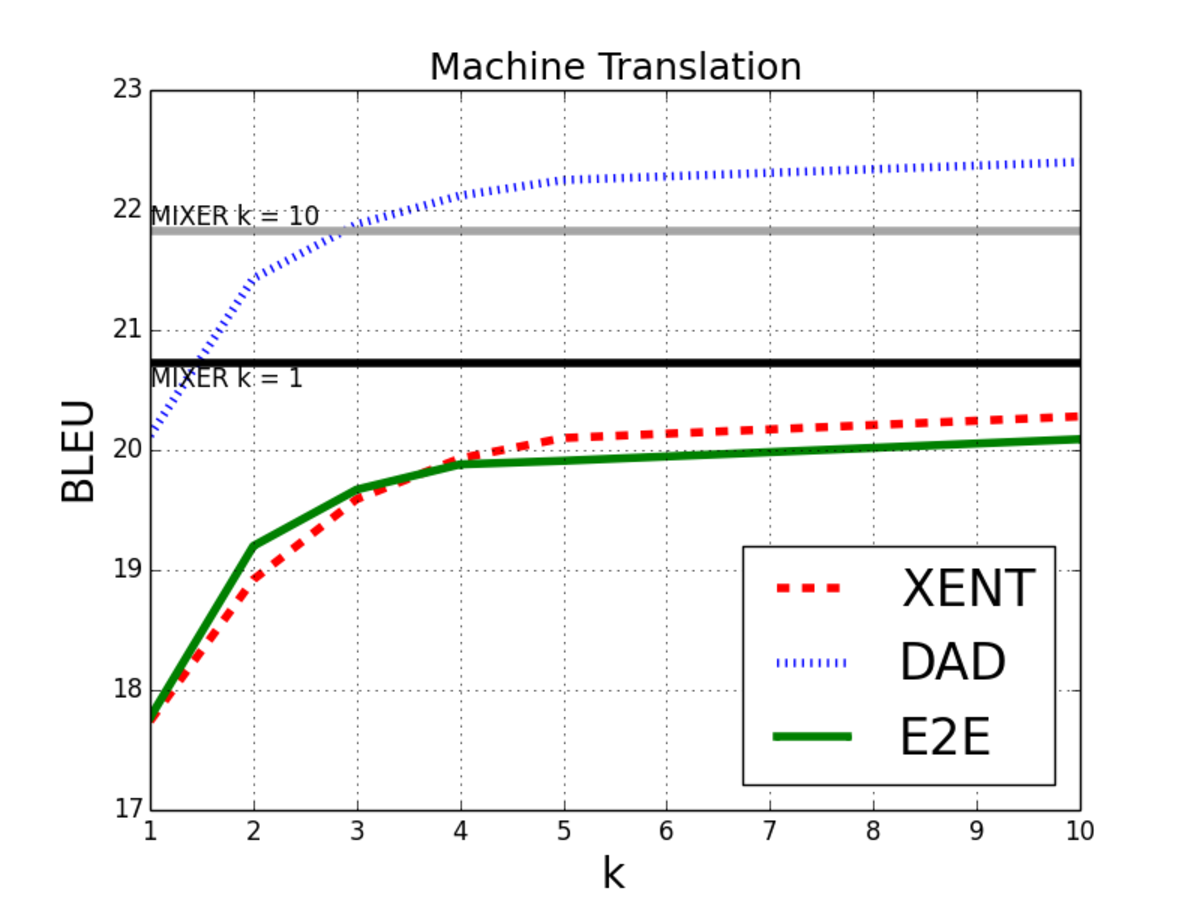
\includegraphics[width=.35\linewidth]{mt_beamsearch.pdf}
 \hspace{-.6cm}
  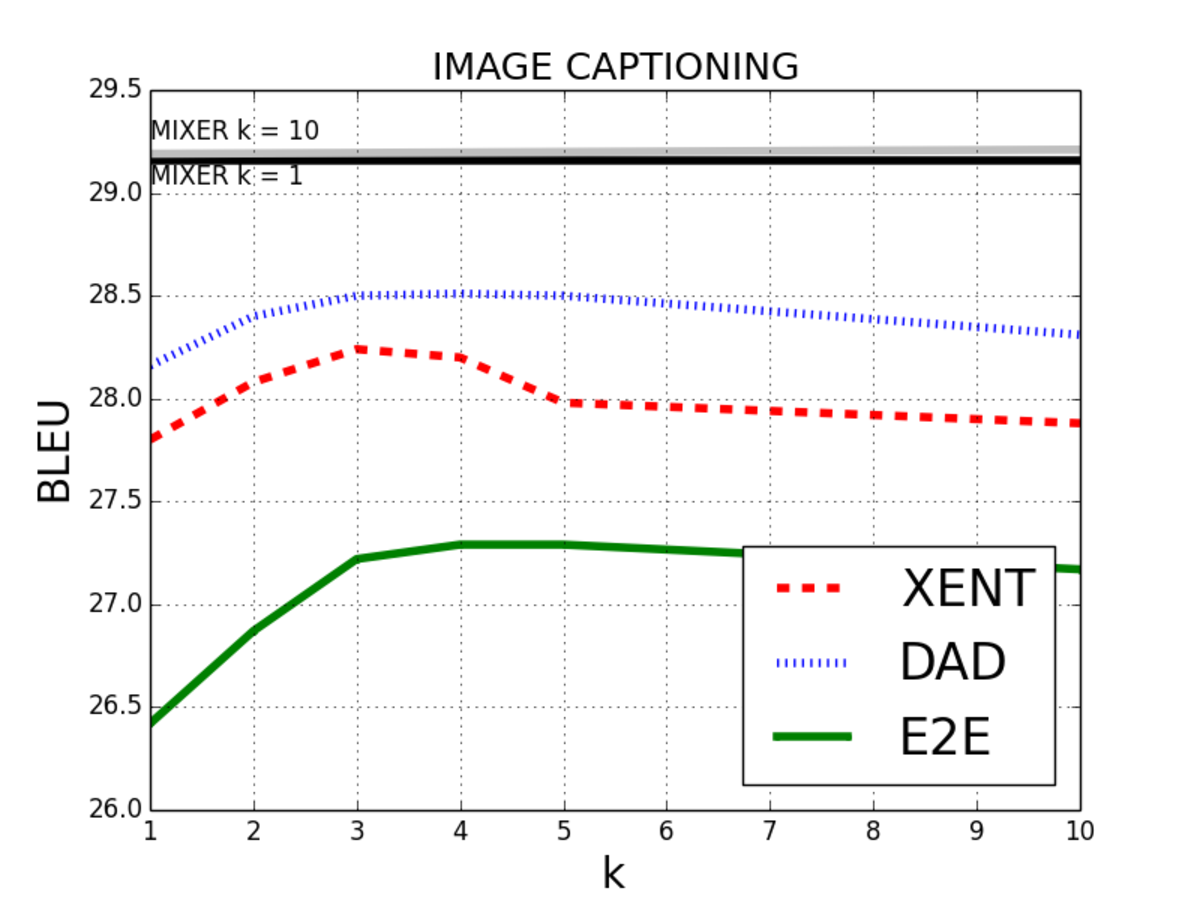
\includegraphics[width=.35\linewidth]{ic_beamsearch.pdf}
\end{center}
\vspace{-.2cm}
\caption{Test score (ROUGE for summarization and BLEU for machine translation and image captioning) as a function of the number of hypotheses $k$ in the beam search. Beam search always improves performance, although the amount depends on the task. The dark line shows the performance of MIXER using greedy generation, while the gray line shows MIXER using beam search with $k=10$.}
% BLEU when increasing the 
\label{fig:beam_search}
\end{figure}

We observe that MIXER produces the best generations and improves generation over XENT by $1$ to $3$ points across all the tasks. 
Unfortunately the E2E approach did not prove to be very effective. Training at the sequence level and directly optimizing for testing score yields better generations than turning a sequence of discrete decisions into a differentiable process amenable to standard back-propagation of the error. 
DAD is usually better than the XENT, but not as good as MIXER.  

Overall, these experiments demonstrate the importance of optimizing for the metric used at test time. In summarization for instance, XENT and MIXER trained with ROUGE achieve a poor performance in terms of BLEU (8.16 and 5.80 versus 9.32 of MIXER trained with BLEU); likewise, MIXER trained with BLEU does not achieve as good ROUGE score as 
a MIXER optimizing ROUGE at training time as well (15.1 versus 16.22, see also Figure~\ref{fig:summarization_bleu_rouge} in Supplementary Material).

Next, we experimented with beam search. The results in Figure~\ref{fig:beam_search} suggest that all methods, including MIXER, improve the quality of their generation by using beam search. However, the extent of the improvement is very much task dependent. We observe that the greedy performance of MIXER (i.e., {\em without} beam search) cannot be matched by baselines using beam search in two out of the three tasks. Moreover, MIXER is several times faster since it relies only on greedy search.

It is worth mentioning that the REINFORCE baseline did not work for these applications. Exploration from a random policy has little chance of success. We do not report it since we were never able to make it converge within a reasonable amount of time. Using the hybrid XENT-REINFORCE loss {\em without} incremental learning is also insufficient to make training take off from random chance. In order to gain some insight on what kind of schedule works, we report in Table~\ref{tab:scheduling} of Supplementary Material the best values we found after grid search over the hyper-parameters of MIXER.
Finally, we report some anecdotal examples of MIXER generation in Figure~\ref{fig:generation} of Supplementary Material. 
%, showing that also qualitatively MIXER generally produces better generations. 
